\chapter{STM32及其编程简介}

\section{STM32是什么}
STM32是指意法半导体(STMicroelectronics)制造的一系列32位ARM架构单片机,这些单片机依据它们使用的核心不同,分为许多系列,例如本文档主要介绍的F1系列采用的是Cortex-M3内核 \footnote{https://en.wikipedia.org/wiki/STM32}。
作为单片机,STM32不仅包含了CPU核,还集成了Flash程序存储器、sRAM内存,以及诸如GPIO控制器的丰富外设,构成了一个片上系统(
\ac{SoC}
)。此外,STM32F1系列单片机的时钟频率可以高达72MHz,远超Arduino UNO的时钟频率,因此可以实现一些复杂的、繁重的控制任务,以及一些常用的算法。
\par 
本文档主要介绍的是STM32F103C8单片机,其中,这个命名包含的信息有:
\begin{itemize}
	\item STM32 - 表示ST生产的32位单片机
	\item F103 - 该单片机的系列
	\item C - 引脚数为48个
	\item 8 - Flash大小为64KiB\footnote{1 KiB = 1024 Bytes}
\end{itemize}
此外,它的内存容量为20KiB,是一款“中密度”单片机产品。
\par 
关于STM32F103C8的更详细的数据可以从它的Datasheet\footnote{https://www.st.com/resource/en/datasheet/stm32f103c8.pdf}中查到,这里不再继续对其进行介绍。

\section{STM32程序怎么写}
虽然我们认为这篇文档的读者以及掌握了基本的C语言程序设计,但是,在一个高度抽象的计算机上编程,与这里为单片机编程有着相当大的区别,所以,我们有必要从本质出发认识STM32程序的设计方法。
\subsection{程序的本质是什么}
程序的本质,当然是计算,毕竟程序是为“计算机”设计的。计算,可以认为是程序唯一的本质,CPU的所有行为不过是从存储介质中取得运算数,按程序对其计算,再将结果写入规定的存储介质中。可是这样,单片机是如何完成各种强大的控制功能的呢?这些功能,实际上是通过逻辑电路来实现的,CPU将控制这些逻辑电路的参数写入规定好的寄存器中,就可以告诉相应的逻辑电路该产生什么行为,除非遭遇了宇宙射线什么的,否则这些逻辑器件总是会乖乖听话。这就是单片机控制功能的来源。
\par 
不如举个例子,查阅STM32的参考手册\footnote{https://www.st.com/resource/en/reference\_manual/cd00171190.pdf}(\ac{RM}),可以知道GPIO这个外设有一个寄存器叫做“ODR (Port output data register)”,可以控制GPIO的输出电平,如下图:
\par 
\begin{figure}[h]
	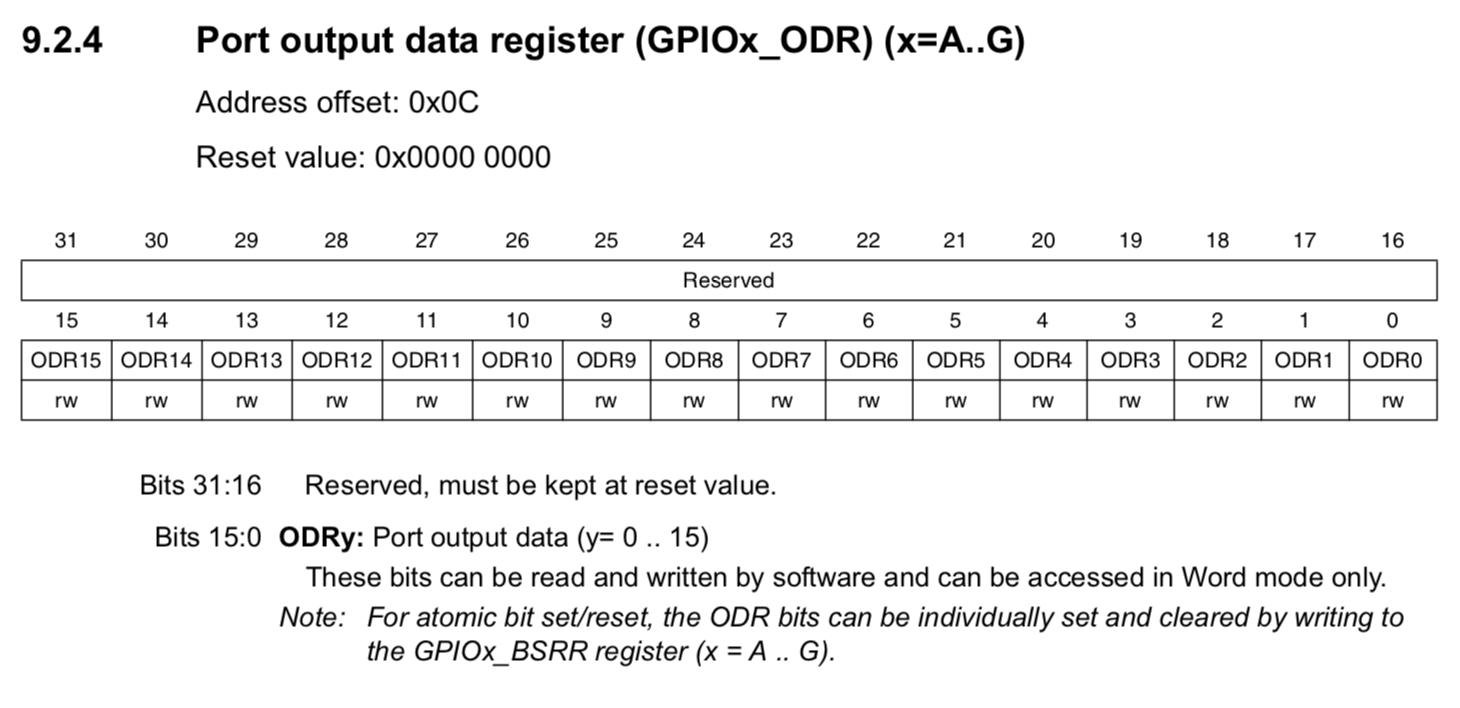
\includegraphics[width=\textwidth]{images/content/ODR.png}
	\captionof{figure}{ODR寄存器}
\end{figure}
\par 
假设GPIOA已经正确初始化,那么只要我们向GPIOA的ODR寄存器写入0x01,就可以控制PA1引脚输出高电平。为此,我们的程序可能长得像下面这样:
\par 
\begin{lstlisting}[language=bash, style=customStyleC, caption=控制PA1输出高电平]
GPIOA->ODR = 0x01;
\end{lstlisting}
\par 
实际上,完成这个操作的确这么简单,这一行程序的功能也没有超出“计算”的范围,因为它就是向一个指定的位置写入了一个预先算好的数据。
\par 
所以我们说,程序的本质是计算。
